% === Datasets ===
\section{Datasets}
\label{sec:datasets}

A faithful evaluation must cover the range a deployed system faces: from richly instrumented services with logs, metrics, and traces down to bare, text-only reports. We therefore use three datasets along this realism spectrum (Table~\ref{tab:datasets}). The first two we \emph{collect and release}: instrumented microservice systems under controlled fault injection, pairing multi-signal telemetry with incident tickets and exact per-window labels. The third we \emph{reuse}: a large corpus of real, engineer-written Apache Jira incidents testing whether methods tuned on synthetic data hold up in the field. The synthetic datasets support exact window-to-ticket evaluation and telemetry-based gating; the real corpus supports large-scale text-only retrieval under noisier, inferred relevance labels.

\begin{table}[t]
\centering
\caption{The three evaluation datasets, spanning fully instrumented synthetic
incidents to real, text-only ones. \emph{Memory} is the pool of past incidents
available for retrieval; \emph{test windows} are the held-out queries used in
\S\ref{sec:results}.}
\label{tab:datasets}
\footnotesize
\setlength{\tabcolsep}{4pt}
\begin{tabular}{lccc}
\toprule
 & Online Boutique & OTel Demo & World of Logs \\
\midrule
Origin           & collected (ours) & collected (ours) & reused~\cite{wang2026worldoflogs} \\
Evidence         & full telemetry   & full telemetry   & text only \\
Scale            & 11 services      & 17 svc.\ + Kafka & 24 projects \\
Fault scenarios  & 26 families      & 52 scenarios     & real incidents \\
Memory incidents & 347              & 147              & 38{,}642 \\
Test windows     & 1{,}008          & 247              & 13{,}388 \\
Split            & by family        & by family        & leave-domain-out \\
\bottomrule
\end{tabular}
\end{table}

\subsection{Collected Telemetry Datasets}
\label{sec:datasets-synthetic}

\begin{figure}[t]
\centering
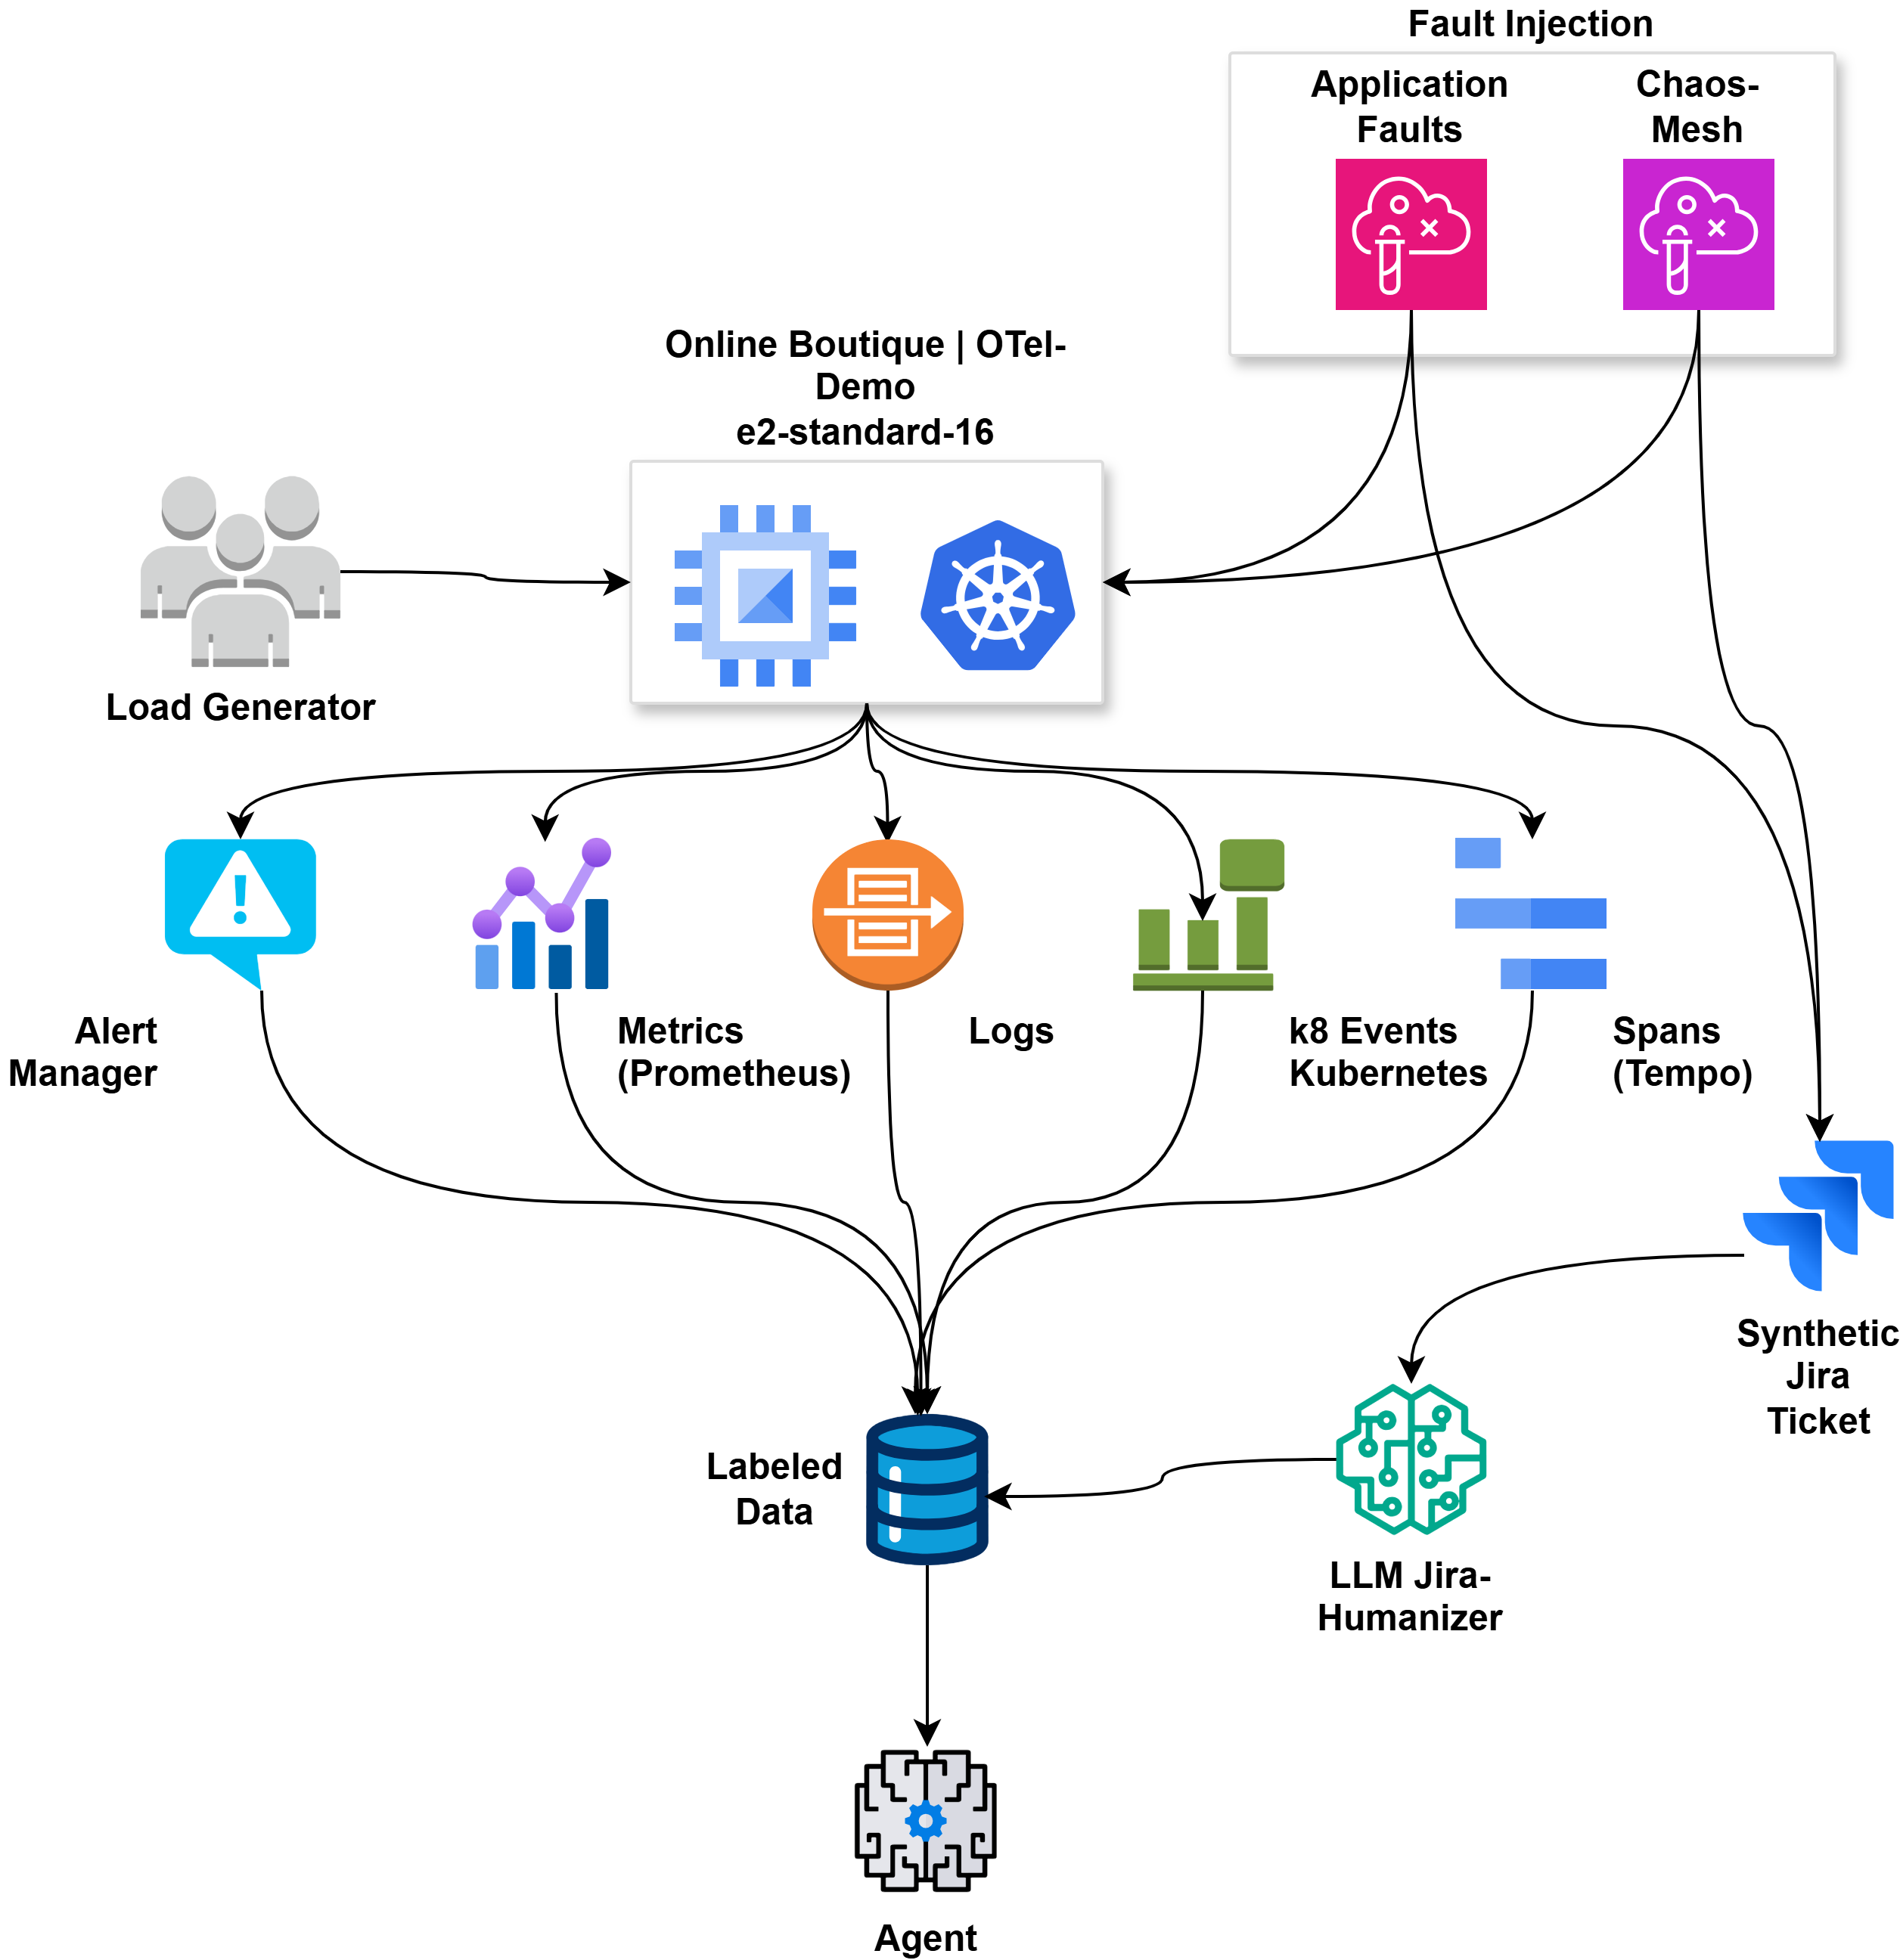
\includegraphics[width=.95\columnwidth]{figures/data-collection.png}
\caption{Data-collection pipeline for the two telemetry datasets. A load
generator exercises an open-source microservice application in Kubernetes while
controlled faults (application-level failures and chaos-engineering network
faults) are injected. The resulting alerts, metrics, logs, cluster events, and distributed-trace spans are captured per window, paired with a synthetic incident ticket (rewritten into engineer voice by a language model) as the retrieval target. The triage system consumes the labelled result.}
\label{fig:collection}
\end{figure}

Both datasets come from a single collection pipeline (Figure~\ref{fig:collection}).
We deploy an open-source microservice application in a Kubernetes cluster
instrumented with a standard observability stack (Prometheus for metrics, Tempo
for distributed traces, and Loki for logs), drive it with a synthetic load
generator, and inject faults under controlled, fully labelled conditions. The
unit of collection is a \emph{scenario}: one fault, injected for a fixed
duration, with its ground truth declared in advance. Each scenario produces three
consecutive \emph{observation windows} (a fault-free baseline just before the
fault, the active fault itself, and a recovery phase after it is cleared), and we
label every window with one of three classes: \textbf{ticket-worthy} (a real
engineer would open an issue), \textbf{borderline} (recovering or marginal), or
\textbf{noise} (normal operation). A window, a short slice of one service's
activity (5 minutes), is the atomic input to the triage system.

For each window we archive everything the platform recorded: the service's logs,
its CPU, memory, and restart series with any firing alerts, the cluster's events
and pod state, and a sample of distributed traces. When a scenario warrants
attention, we generate the incident ticket and rewrite it with a language model
into natural, engineer-voice prose, so the memory reads like real filed tickets;
this ticket is the retrieval target. Because we control the
injection, the window--ticket link is \emph{exact ground truth} rather than
inferred. We also record realistic near-misses (a service stressed but never
failing, warranting no page) and \emph{orphan} faults (genuine ticket-worthy
failures for which no ticket is filed, so a page-worthy window has no precedent in
memory). The near-misses separate a useful triage system from one that pages
constantly; the orphans test whether it recognizes an incident from telemetry
rather than only when a matching ticket exists.

\textbf{Online Boutique}~\cite{googleboutique} is an eleven-service e-commerce demo
spanning five languages; its 26 fault families include hard service outages (e.g., scaling a service to zero replicas), latency and resource-pressure
degradations such as slow memory and connection leaks, pod restarts, network
faults injected with a chaos-engineering tool~\cite{chaosmesh} (partitions, packet
loss, DNS failures), and deployment churn. \textbf{OpenTelemetry
Demo}~\cite{oteldemo} adds architectural distance:
seventeen services in twelve languages, organized around a Kafka message bus with
asynchronous downstream consumers. Its 52 scenarios extend from single-service faults (triggered through the application's built-in failure switches) to Kafka-specific failures such as broker outages and consumer lag with no Online Boutique analogue, and on to concurrent and cascading multi-fault episodes. Together the two contribute roughly $6{,}700$ and $1{,}600$ labelled
windows and tens of gigabytes of raw telemetry, which we release as self-contained
archives. Within each dataset we hold out whole fault families for testing, so test
windows never come from a scenario seen during training.

\subsection{Real-World Incidents: World of Logs}
\label{sec:datasets-wol}

To see whether a method survives contact with reality, we turn to the \emph{World
of Logs} collection~\cite{wang2026worldoflogs}, a public archive of logs and issue reports
mined from online software-engineering sources, including public Jira trackers.
This dataset is not our contribution; we derive an evaluation slice from its Apache Jira issues. We select 24 of its
distributed-systems projects (message brokers, datastores, stream processors,
the Hadoop ecosystem, and others), which together provide a memory of $38{,}642$
resolved bug reports to retrieve from and $78{,}140$ incident queries to triage.
Each query receives the same three labels as our synthetic data, assigned
automatically from the ticket's type and final resolution: a fixed bug is
ticket-worthy, an engaged-but-inconclusive outcome is borderline, and a rejected
or non-bug issue is noise.

This corpus is deliberately the hardest of the three, for two reasons. It is
\emph{text only}: authentic, terse, engineer-written descriptions with no
telemetry whatsoever, exactly the degraded regime to which our controller must
fall back. And we evaluate it under a \emph{leave-domain-out} split, holding out
two entire project families (a message broker and a database engine, $13{,}388$
incidents) so the system must match incidents in projects it never saw while training. 

The counts serve different roles. The 78,140 Jira issues form the labelled triage pool before the held-out-domain split. Table I reports the 13,388 held-out issues used as test windows for end-to-end triage. Retrieval metrics are computed only on held-out fixed-bug queries that have at least one eligible past match under the inferred relation; this yields 5,150 retrieval queries in Table II. Borderline and noise issues are retained for triage evaluation but excluded from Hit@k and MRR because they have no relevant prior incident by construction.

Real incidents come with no manually curated answer key linking each query to the past ticket that would best support triage, so we use an inferred matching relation: a query and a past ticket match when they share a project and at least one software component, with a stricter variant that also requires overlapping symptom terms. We report retrieval quality under both relations and, because inferred labels deserve scrutiny, separately validate them with an LLM-as-judge check (\S\ref{sec:results}). Only genuine bug reports have matches; borderline and
noise queries have none by construction and are excluded from the retrieval
measurements.

\smallskip
\noindent\textbf{Component metadata is load-bearing, so we characterize it.}
Because the relation is defined on the \texttt{project} and \texttt{components}
fields, the quality and coverage of those fields bound what the metric can mean.
Across all $78{,}140$ issues, $75.3\%$ carry at least one component ($80.5\%$ on
the test split); most carry exactly one ($48{,}394$ issues) or two ($8{,}935$).
Vocabularies are project-local and very uneven, from $205$ distinct components in
Camel to $9$ in IMPALA, and they are not a clean taxonomy: alongside subsystem
names they include release numbers such as \texttt{10.3} and \texttt{2.2.1}, so
two issues can share a ``component'' only by sharing a version.

This directly conditions the evaluation, and we state the consequence plainly
rather than leaving it to be inferred from a table. Of the $6{,}773$ held-out
ticket-worthy queries, $1{,}621$ ($23.9\%$) carry no component at all and
therefore have no gold match by construction. The retrieval results in
\S\ref{sec:results} are computed on the remaining $5{,}150$, and the strict
relation reduces this further to $4{,}362$. Our real-corpus retrieval numbers are
thus conditioned on issues whose authors filled in component metadata, a
non-random three quarters of ticket-worthy issues, and they should be read as
describing that subpopulation rather than all real incidents.
